\section{Auswertung}
\label{sec:Auswertung}
\subsection{Bestimmung der Güteziffer}
In Tabelle \ref{tab:tabe1} sind die gemessen Werte der Wärmepumpe aufgeführt.
\begin{table}[H]
  \centering
  \caption{Messwerte der Wärmepumpe}
  \label{tab:tabe1}
    \begin{tabular}{S S S S S S}
    \toprule
    $ t  \: / \si{\second} $ & $ p_a \: / \si{\bar} $ & $ p_b \: / \si{\bar} $ &
    $ T_1 \: / \si{\kelvin} $ & $ T_2 \: / \si{\kelvin} $ & $ P \: / \: \si{\watt} $\\
    \midrule
    0 & 5.0 & 5.0 & 293.65 & 293.65 & 0 \\
    60 & 4.7 & 6.0 & 294.15 & 293.55 & 115 \\
    120 & 4.4 & 6.4 & 295.15 & 293.15 & 118 \\
    180 & 4.5 & 6.9 & 296.35 & 291.95 & 122 \\
    240 & 4.6 & 7.0 & 297.55 & 290.95 & 125 \\
    300 & 4.6 & 7.0 & 298.85 & 289.95 & 125 \\
    360 & 4.5 & 7.2 & 300.05 & 289.15 & 123 \\
    420 & 4.4 & 7.4 & 301.15 & 288.45 & 123 \\
    480 & 4.3 & 7.8 & 302.35 & 287.65 & 122 \\
    540 & 4.2 & 8.0 & 303.55 & 286.95 & 122 \\
    600 & 4.2 & 8.1 & 304.65 & 286.25 & 121 \\
    660 & 4.1 & 8.3 & 305.75 & 285.55 & 121 \\
    720 & 4.0 & 8.5 & 306.75 & 284.95 & 121 \\
    780 & 4.0 & 8.8 & 307.75 & 284.35 & 121 \\
    840 & 3.9 & 9.0 & 308.75 & 283.75 & 121 \\
    900 & 3.8 & 9.1 & 309.65 & 283.15 & 121 \\
    960 & 3.8 & 9.2 & 310.55 & 282.55 & 122 \\
    1020 & 3.8 & 9.5 & 311.45 & 282.05 & 122 \\
    1080 & 3.7 & 9.8 & 312.25 & 281.55 & 122 \\
    1140 & 3.7 & 10.0 & 313.05 & 281.15 & 122 \\
    1200 & 3.7 & 10.0 & 313.9 & 280.65 & 122 \\
    1260 & 3.6 & 10.2 & 314.65 & 280.25 & 123 \\
    1320 & 3.6 & 10.3 & 315.35 & 279.85 & 123 \\
    1380 & 3.6 & 10.6 & 316.15 & 279.45 & 124 \\
    1440 & 3.6 & 10.8 & 316.85 & 279.15 & 124 \\
    1500 & 3.6 & 11.0 & 317.55 & 278.75 & 124 \\
    1560 & 3.6 & 11.1 & 318.25 & 278.55 & 124 \\
    1620 & 3.6 & 11.2 & 318.95 & 278.25 & 125 \\
    1680 & 3.5 & 11.4 & 319.55 & 277.95 & 125 \\
    1740 & 3.5 & 11.5 & 320.15 & 277.65 & 125 \\
    1800 & 3.5 & 11.7 & 320.75 & 277.45 & 125 \\
    1860 & 3.5 & 11.9 & 321.35 & 277.25 & 125 \\
    1920 & 3.5 & 12.0 & 321.95 & 277.05 & 125 \\
    1980 & 3.5 & 12.1 & 322.45 & 276.95 & 125 \\








      \bottomrule
    \end{tabular}
\end{table}

\noindent Die Temperaturverläufe von $ T_1 $ (warmes Reservoir) und $ T_2 $ (kaltes
Reservoir) sind in Abbildung \ref{fig:plot1} in Abhängigkeit der Zeit dargestellt.
\begin{figure}[H]
  \centering
  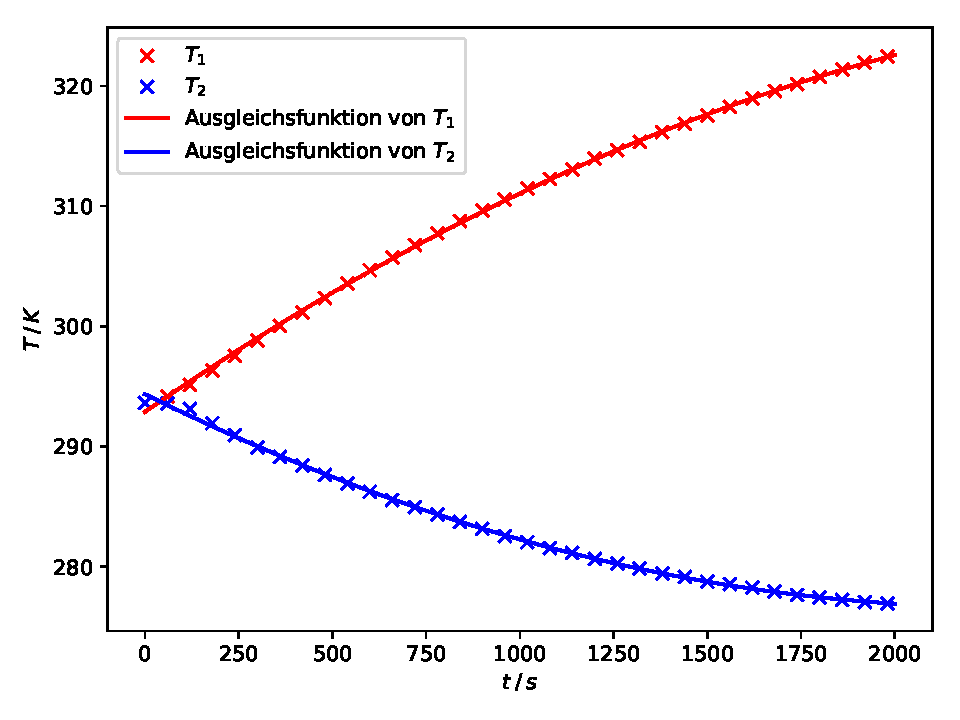
\includegraphics{plot1.pdf}
  \caption{Messwerte und Ausgleichsfunktionen der Temperaturverläufe}
  \label{fig:plot1}
\end{figure}
Die Augleichsfunktionen wurde durch eine Ausgleichsrechung mit der Funktion
\begin{equation}
  T(t) = at^2 +bt +c
\end{equation}
erstellt, wobei sich bei dem wärmeren Reservoir die Parameter
\begin{align*}
  a_w &= (-33,3 \: \pm \: 1,0) \cdot 10^{-7} \: \si{\kelvin\per\second\squared}\\
  b_w &= (21,50 \: \pm \: 0,21) \cdot 10^{-3} \: \si{\kelvin\per\second}\\
  c_w &= (292.882 \: \pm \: 0,091) \: \si{\kelvin} \\
\end{align*}
und bei dem kälteren Reservoir die Parameter
\begin{align*}
  a_k &= (33,7 \: \pm \: 1,0) \cdot 10^{-7} \: \si{\kelvin\per\second\squared}\\
  b_k &= (-15,44 \: \pm \: 0,21) \cdot 10^{-3} \: \si{\kelvin\per\second}\\
  c_k &= (294.349 \: \pm \: 0,088) \: \si{\kelvin}\\
\end{align*}
ergeben.

Um den Differentialquotienten zu bilden, wird die Funktion T(t) nun nach t abgeleitet, sodass
sich
\begin{equation}
  \frac{d T(t)}{d t} = 2at +b
\end{equation}
ergibt.
Werden nun die entsprechenden Parameter, sowie die vier beliebig gewählten Zeiten
$t_1 = \SI{480}{\second}$, $t_2 = \SI{960}{\second}$, $t_3 = \SI{1500}{\second}$
und $t_4 = \SI{1980}{\second}$ eingesetzt, ergeben sich die jeweiligen Differentialquotienten.
\begin{table}[H]
  \centering
  \caption{Wertetabelle für $\alpha$ und $C_V$.}
  \label{tab:tab2}
    \begin{tabular}{S S S S S}
    \toprule
    $ T\: \text{in}\: \si{\K} $ & $ {\alpha \cdot 10^{-6} \: \text{in}\: \si {\per\K}} $ &
    $ C_V \: \text{in}\: \si{\J\per\K\mol} $\\
    \midrule %Cv, a *10-6, Cv
    %0 & 1 & 1\\
    88.60\pm0.24 & 9.56\pm0.06 & 14.17\pm8.13  \\ %&3.6 & 318.97\pm0.85\\
    93.81\pm0.24 & 10.10\pm0.06 & 17.58\pm10.03 \\ %& 4.7 & 440.90\pm1.11\\
    99.74\pm0.24 & 10.66\pm0.05 & 15.52\pm8.84 \\ %& 5.1 & 508.68\pm1.21\\
    104.74\pm0.24 & 11.07\pm0.05 & 18.44\pm10.52 \\ %& 4.6 & 481.79\pm1.09\\
    110.94\pm0.24 &  11.54\pm0.05 & 14.86\pm8.45 \\ %& 5.3 & 587.97\pm1.27\\
    115.96\pm0.24 & 11.89\pm0.05 & 18.49\pm10.52 \\ %& 4.6 & 533.41\pm1.10\\
    121.47\pm0.24 &  12.22\pm0.05 & 16.83\pm9.57 \\ %& 4.9 & 595.21\pm1.17\\
    126.99\pm0.24 & 12.53\pm0.04 & 16.79\pm9.54 \\ %& 4.9 & 622.29\pm1.18\\
    131.58\pm0.24 & 12.77\pm0.04 & 20.42\pm11.62 \\ %& 4.2 & 552.62\pm1.01\\
    136.65\pm0.24 & 13.02\pm0.04 & 18.40\pm10.47 \\ %& 4.6 & 628.57\pm1.11\\
    141.49\pm0.24 & 13.24\pm0.04 & 19.28\pm10.97 \\ %& 4.4 & 622.54\pm1.07\\
    146.34\pm0.24 & 13.44\pm0.04 & 19.24\pm10.95 \\ %& 4.4 & 643.88\pm1.07\\
    150.95\pm0.24 & 13.62\pm0.04 & 20.22\pm11.52 \\ %& 4.3 & 649.11\pm1.05\\
    155.34\pm0.24 & 13.79\pm0.04 & 21.31\pm12.14 \\ %& 4.1 & 636.88\pm0.98\\
    159.97\pm0.24 & 13.95\pm0.04 & 20.12\pm11.47 \\ %& 4.3 & 687.89\pm1.05\\
    164.62\pm0.24 & 14.10\pm0.04 & 20.18\pm11.51 \\ %& 4.3 & 707.87\pm1.06\\
    168.79\pm0.25 & 14.23\pm0.04 & 22.54\pm12.86 \\ %& 3.9 & 658.27\pm0.95\\
    173.45\pm0.25 &  14.37\pm0.04 & 20.08\pm11.46 \\ %& 4.3 & 745.84\pm1.06\\
    178.13\pm0.25 &  14.50\pm0.04 & 20.04\pm11.44 \\ %& 4.3 & 765.94\pm1.06\\
    182.56\pm0.25 &  14.62\pm0.04 & 21.11\pm12.06\\
    192.70\pm0.25 &  14.87\pm0.04 & 18.41\pm10.47\\
    200.15\pm0.25 &  15.04\pm0.04 & 25.19\pm14.28\\
    208.87\pm0.25 &  15.23\pm0.04 & 21.43\pm12.18\\
    217.12\pm0.25 &  15.38\pm0.04 & 22.65\pm12.88\\
    225.15\pm0.25 &  15.53\pm0.03 & 23.27\pm13.24\\
    232.70\pm0.25 &  15.70\pm0.03 & 24.75\pm14.08\\
    240.53\pm0.25 &  15.74\pm0.03 & 23.84\pm13.58\\
    248.39\pm0.25 &  15.89\pm0.03 & 23.74\pm13.53& \\
    256.01\pm0.25 &  15.97\pm0.03 & 24.46\pm13.94 \\
    263.41\pm0.26 &  16.01\pm0.03 & 25.22\pm14.38 \\
    271.08\pm0.26 &  16.18\pm0.03 & 24.26\pm13.86 \\
    278.52\pm0.26 &  16.27\pm0.03 & 25.03\pm14.29&\\
    285.98\pm0.26 &  16.35\pm0.03 & 24.92\pm14.25 \\
    293.21\pm0.26 &  16.42\pm0.03 & 25.74\pm14.72 \\
    300.98\pm0.26 &  16.50\pm0.03 & 23.87\pm13.68 \\
    308.51\pm0.26 &  16.57\pm0.03 & 24.63\pm14.12\\



      \bottomrule
    \end{tabular}
\end{table}

Die Fehler berechnen sich hierbei aus den Fehlern der Ausgleichsrechnung durch die Gauß´sche
Fehlerfortpflanzung
\begin{equation}
  \increment f = \sqrt{ \sum_{i=1}^N \left( \frac{\partial f}{\partial x_i}\right)^2
  \cdot (\increment x_i)^2  } \: .
  \label{eqn:gaus}
\end{equation}
Also in diesem Fall:
\begin{equation}
  \increment \frac{d T(t)}{d t} = \sqrt{(2t)^2 \cdot (\increment a)^2 + (\increment b)^2 } \: .
  \label{eqn:f1}
\end{equation}
\\
\\
\noindent Um die Güteziffer zu bestimmen, wird Gleichungen \ref{eqn:güte3} verwendet,
wobei die spezifischen Wärmekapazität von Wasser $\SI{4183}{\joule\per\kilo\gram\per\kelvin}$ \cite{chemie}
beträgt, die Masse des Wassers $\SI{4}{\kilo\gram}$ und die Wärmekapazität des Kupfers
$\SI{750}{\joule\per\kelvin}$. Die entsprechende Leistung kann in der Tabelle \ref{tab:tabe1}
abgelesen werden.
Die Fehler berechnen sich hierbei nach Gleichung \ref{eqn:gaus} durch
\begin{equation}
  \increment v_{\text{real}} = \sqrt{\left(\frac{m_1c_w +m_2c_k}{N}\right)^2 \cdot \left(\increment \frac{d T(t)_1}{d t}\right)^2} \: .
  \label{eqn:f2}
\end{equation}
Die Theoriewerte für die ideale Wärmepumpe berechnen sich dabei durch die Gleichung
\ref{eqn:güte2} (die Temperatur muss zunächst noch in Kelvin umgerechnet werden) und die Abweichungen durch
\begin{equation*}
  \frac{\lvert \text{Wert}_{\text{Messung}}-\text{Wert}_{\text{Theorie}}\rvert}{\text{Wert}_{\text{Theorie}}} \: .
\end{equation*}
Somit ergibt sich insgesamt für die jeweils entsprechenden Differentialquotienten:
\begin{table}
  \centering
  \caption{Messwerte für den ersten Doppelspalt.}
   \begin{tabular}{S S| S S | S S}
    \toprule
    $x/\; \si{\mm}$& $A/\;\si{\nA}$ &
    $x/\; \si{\mm}$& $A/\;\si{\nA}$ &
    $x/\; \si{\mm}$& $A/\;\si{\nA}$ \\
    \midrule

    15.0& 4.6& 23.0& 25.0& 29.5& 6.0\\
    15.5& 4.2& 23.5& 30.0& 30.0& 5.3\\
    16.0& 4.0& 24.0& 35.0& 30.5& 4.9\\
    16.5& 4.0& 24.25& 36.0& 31.0& 4.7\\
    17.0& 4.4& 24.5& 37.0& 31.5& 4.4\\
    17.5& 5.5& 24.75& 38.0& 32.0& 4.2\\
    18.0& 6.6& 25.00& 37.0& 32.5& 3.8\\
    18.5& 7.7& 25.25& 36.0& 33.0& 3.6\\
    19.0& 8.2& 25.5& 36.0& 33.5& 3.2\\
    19.5& 8.4& 26.0& 33.0& 34.0& 3.2\\
    20.0& 8.4& 26.5& 28.5& 34.5& 3.2\\
    20.25& 8.4& 27.0& 23.0& 35.0& 3.3\\
    20.5& 8,7& 27.5& 18.0& 35.5& 3.4\\
    21.0& 9.8& 28.0& 13.5& 36.0& 3.5\\
    21.5& 12.0& 28.5& 10.0\\
    22.0& 15.0& 29.0& 7.8\\
    22.5& 20.0& 29.25& 6.7\\


   \bottomrule
  \end{tabular}
  \label{tab:tabelle3}
\end{table}


\subsection{Bestimmung des Massendurchsatzes}
Um den Massendurchsatz zu bestimmen, wird zunächst die Verdampfungswärme L des
verwendeten Gases bestimmt.
Hierzu wird zunächst der Logarithmus des Verhältnisses $\frac{p_b}{p_0}$ gebildet
(Annahme: $p_0 \approx \SI{1}{\bar}$), was daraufhin gegen den Kehrwert der Temperatur $T_1$
aufgetragen wird. Dann wird eine lineare Ausgleichsrechnung der Form $ f(x) =ax +b$ durchgeführt, wie in
Abbildung \ref{fig:plot2} zu sehen ist.
\begin{figure}[H]
  \centering
  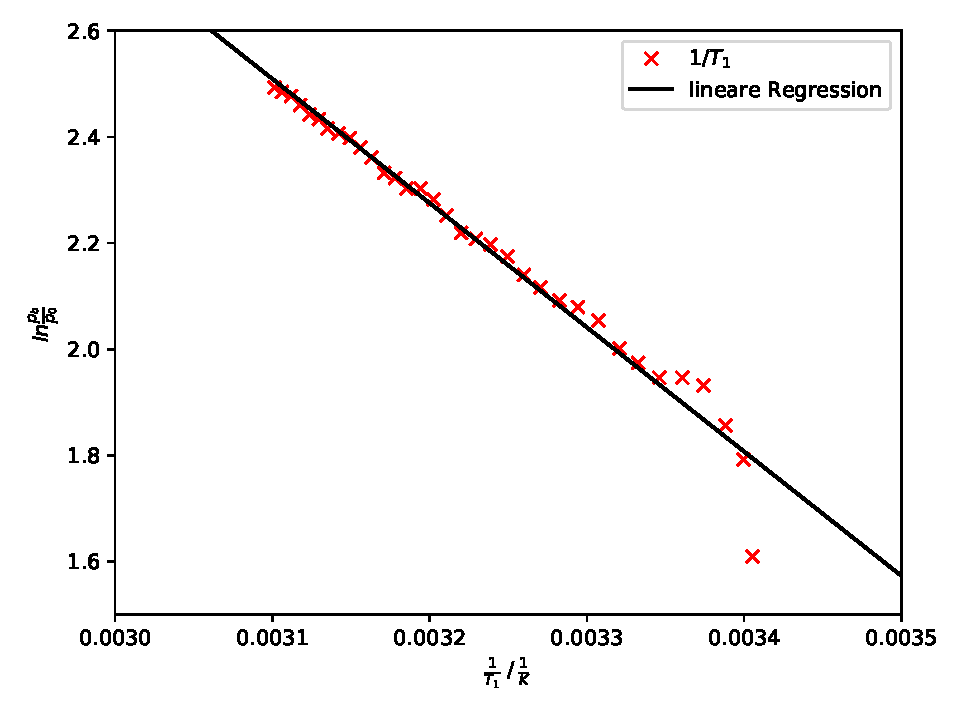
\includegraphics{plot2.pdf}
  \caption{Dampfdruckkurve mit linearer Regression}
  \label{fig:plot2}
\end{figure}
Hieraus ergeben sich die Parameter
\begin{align*}
  a= (-2340 &\pm 69) \: \si{\kelvin} \\
  b= (9,77 &\pm 0,22) \\
\end{align*}
und für die Verdampfungswärme ergibt sich
\begin{equation*}
  L= -a*R = \SI{19.46(58)e3}{\joule\per\mol}
\end{equation*}
wobei R= $\SI{8.3144}{\joule\per\mol\per\kelvin}$ \cite{chemie2} die allgemeine Gaskonstante ist.
Der Fehler berechnet sich durch
\begin{equation}
  \increment L = \sqrt{\left(-R\right)^2 \cdot \left(\increment a\right)^2} \: .
  \label{eqn:f2}
\end{equation}
Aus Gleichung \ref{eqn:masse} und einer molaren Masse von $\SI{120.91}{\gram\per\mol}$
\cite{chemie3} folgt:
\begin{table}[H]
  \centering
   \begin{tabular}{c c c c}
    \toprule
    Nummer der Oberwelle & $ U_{\text Theorie,Rechteck}\: / \si{\volt} $ &
    $ U_{\text Theorie,Dreick}\: / \si{\volt} $ & $ U_{\text Theorie,Sägezahn}\: / \si{\volt} $ \\
    \midrule
    1 & 1145 & 182 & 573 \\
    2 & 0 & 0 & 286 \\
    3 & 573 & 20 & 191 \\
    4 & 0 & 0 & 143 \\
    5 & 229 & 7 & 115 \\
    6 & 0 & 0 & 96 \\
    7 & 164 & 4 & 82 \\
    8 & 0 & 0 & 72 \\
    9 & 127 & 2 & 64 \\
    10 & 0 & 0 & 57 \\
    \bottomrule
  \end{tabular}
  \caption{Eingestellte Schwingungsamplituden.}
  \label{tab:tabe4}
\end{table}

Die Fehler berechenen sich hierbei durch:
\begin{equation}
  \increment \frac{dm}{dt} = \sqrt{\left(\frac{1}{L^2}(m_2c_w+m_kc_k) \frac{d T_2}{dt} \right)^2 \cdot \left(\increment L\right)^2
  + \left(\frac{1}{L}(m_2c_w+m_kc_k)\right)^2 \cdot \left(\increment \frac{d T_2}{dt} \right)^2}} \: .
  \label{eqn:f3}
\end{equation}
\subsection{Bestimmung der mechanischen Kompressorleistung}
Die Werte zur Berechnung der mechanischen Kompressorleistung lauten:
\begin{align*}
  \kappa &= 1,14 \\
  \rho_0 &= \SI{5.51}{\gram\per\liter} \\
  T_0 &= \SI{20.5}{\celsius}
\end{align*}
Zunächst muss hierzu noch die Dichte $\rho$ bestimmt werden, wobei mit der idealen Gasgleichung
die Gleichung
\begin{equation}
  pV =nRT \iff \frac{pV}{T}{nR}
\end{equation}
folgt. Aus $n_1R =n_2R$ folgt nun
\begin{equation}
  \frac{p_0 V_0}{T_0} = \frac{p_2 V_2}{T_2}
\end{equation}
und mit $\rho = \frac{m}{V}$, $\rho_2=\rho$ und $p_2 =p_a$ schlussendlich:
\begin{equation}
  \frac{p_0}{T_0\rho_0} = \frac{p_a}{T_2 \rho} \iff \rho = \frac{\rho_0 T_0 p_a}{T_2p_0}
\end{equation}
Wird dies in Gleichung \ref{eqn:Nmech}, sowie die Werte für $p_a$ und $p_b$ aus Tabelle
\ref{tab:tabe1} eingesetzt, ergibt sich somit:
\begin{table}[H]
  \centering
  \caption{Bohrung 1 und 2, Vergleich der Sonden mit 1\;MHz und 2\;MHz.}
  \label{tab:tab5}
    \begin{tabular}{c c c c}
    \toprule
    Bohrung & $S_{\text{2\;MHz}}$/\;mm & $S_{\text{ 1\;MHz}}$/\;mm\\
    \midrule
    1 & 1,82 & 2,12\\
    2 & 1,83 & 1,97\\
    \bottomrule
    \end{tabular}
  \end{table}

Die Fehlerrechnung erfolgt hierbei durch \ref{eqn:gaus} mit
\begin{equation}
  \increment N_{\text{mech}} = \sqrt{\left(\frac{1}{\kappa-1}\Biggl(p_{b}\sqrt[\kappa]{\frac{p_{a}}{p_{b}}}-p_{a}\Biggr)
  \frac{\rho_0 T_0 p_a}{T_2p_0}\right)^2 \cdot \left(\increment \frac{dm}{dt} \right)^2} \: .
  \label{eqn:f4}
\end{equation}
